% Options for packages loaded elsewhere
\PassOptionsToPackage{unicode}{hyperref}
\PassOptionsToPackage{hyphens}{url}
\PassOptionsToPackage{dvipsnames,svgnames,x11names}{xcolor}
%
\documentclass[
  12pt,
]{article}
\title{\hfill\break
\hfill\break
\hfill\break
\vspace{1cm}Health club customer dropout membership\footnote{Corresponding address: \href{mailto:sobreiro@esdrm.ipsantarem.pt}{\nolinkurl{sobreiro@esdrm.ipsantarem.pt}}. Quality of Life Research Centre, Polytechnic Institute of Santarém, Portugal}\vspace{0.5cm}}
\author{Pedro Sobreiro, Javier Berrocal, Domingos Martinho, José Garcia Alonso\\
\strut \\
Extremadura University\\}
\date{\hfill\break
\hfill\break
21 julho, 2022\\
\strut \\}

\usepackage{amsmath,amssymb}
\usepackage{lmodern}
\usepackage{setspace}
\usepackage{iftex}
\ifPDFTeX
  \usepackage[T1]{fontenc}
  \usepackage[utf8]{inputenc}
  \usepackage{textcomp} % provide euro and other symbols
\else % if luatex or xetex
  \usepackage{unicode-math}
  \defaultfontfeatures{Scale=MatchLowercase}
  \defaultfontfeatures[\rmfamily]{Ligatures=TeX,Scale=1}
  \setmainfont[]{Times New Roman}
  \setsansfont[]{Times New Roman}
\fi
% Use upquote if available, for straight quotes in verbatim environments
\IfFileExists{upquote.sty}{\usepackage{upquote}}{}
\IfFileExists{microtype.sty}{% use microtype if available
  \usepackage[]{microtype}
  \UseMicrotypeSet[protrusion]{basicmath} % disable protrusion for tt fonts
}{}
\makeatletter
\@ifundefined{KOMAClassName}{% if non-KOMA class
  \IfFileExists{parskip.sty}{%
    \usepackage{parskip}
  }{% else
    \setlength{\parindent}{0pt}
    \setlength{\parskip}{6pt plus 2pt minus 1pt}}
}{% if KOMA class
  \KOMAoptions{parskip=half}}
\makeatother
\usepackage{xcolor}
\IfFileExists{xurl.sty}{\usepackage{xurl}}{} % add URL line breaks if available
\IfFileExists{bookmark.sty}{\usepackage{bookmark}}{\usepackage{hyperref}}
\hypersetup{
  colorlinks=true,
  linkcolor={Maroon},
  filecolor={Maroon},
  citecolor={Blue},
  urlcolor={Blue},
  pdfcreator={LaTeX via pandoc}}
\urlstyle{same} % disable monospaced font for URLs
\usepackage[margin = 1in]{geometry}
\usepackage{color}
\usepackage{fancyvrb}
\newcommand{\VerbBar}{|}
\newcommand{\VERB}{\Verb[commandchars=\\\{\}]}
\DefineVerbatimEnvironment{Highlighting}{Verbatim}{commandchars=\\\{\}}
% Add ',fontsize=\small' for more characters per line
\usepackage{framed}
\definecolor{shadecolor}{RGB}{248,248,248}
\newenvironment{Shaded}{\begin{snugshade}}{\end{snugshade}}
\newcommand{\AlertTok}[1]{\textcolor[rgb]{0.94,0.16,0.16}{#1}}
\newcommand{\AnnotationTok}[1]{\textcolor[rgb]{0.56,0.35,0.01}{\textbf{\textit{#1}}}}
\newcommand{\AttributeTok}[1]{\textcolor[rgb]{0.77,0.63,0.00}{#1}}
\newcommand{\BaseNTok}[1]{\textcolor[rgb]{0.00,0.00,0.81}{#1}}
\newcommand{\BuiltInTok}[1]{#1}
\newcommand{\CharTok}[1]{\textcolor[rgb]{0.31,0.60,0.02}{#1}}
\newcommand{\CommentTok}[1]{\textcolor[rgb]{0.56,0.35,0.01}{\textit{#1}}}
\newcommand{\CommentVarTok}[1]{\textcolor[rgb]{0.56,0.35,0.01}{\textbf{\textit{#1}}}}
\newcommand{\ConstantTok}[1]{\textcolor[rgb]{0.00,0.00,0.00}{#1}}
\newcommand{\ControlFlowTok}[1]{\textcolor[rgb]{0.13,0.29,0.53}{\textbf{#1}}}
\newcommand{\DataTypeTok}[1]{\textcolor[rgb]{0.13,0.29,0.53}{#1}}
\newcommand{\DecValTok}[1]{\textcolor[rgb]{0.00,0.00,0.81}{#1}}
\newcommand{\DocumentationTok}[1]{\textcolor[rgb]{0.56,0.35,0.01}{\textbf{\textit{#1}}}}
\newcommand{\ErrorTok}[1]{\textcolor[rgb]{0.64,0.00,0.00}{\textbf{#1}}}
\newcommand{\ExtensionTok}[1]{#1}
\newcommand{\FloatTok}[1]{\textcolor[rgb]{0.00,0.00,0.81}{#1}}
\newcommand{\FunctionTok}[1]{\textcolor[rgb]{0.00,0.00,0.00}{#1}}
\newcommand{\ImportTok}[1]{#1}
\newcommand{\InformationTok}[1]{\textcolor[rgb]{0.56,0.35,0.01}{\textbf{\textit{#1}}}}
\newcommand{\KeywordTok}[1]{\textcolor[rgb]{0.13,0.29,0.53}{\textbf{#1}}}
\newcommand{\NormalTok}[1]{#1}
\newcommand{\OperatorTok}[1]{\textcolor[rgb]{0.81,0.36,0.00}{\textbf{#1}}}
\newcommand{\OtherTok}[1]{\textcolor[rgb]{0.56,0.35,0.01}{#1}}
\newcommand{\PreprocessorTok}[1]{\textcolor[rgb]{0.56,0.35,0.01}{\textit{#1}}}
\newcommand{\RegionMarkerTok}[1]{#1}
\newcommand{\SpecialCharTok}[1]{\textcolor[rgb]{0.00,0.00,0.00}{#1}}
\newcommand{\SpecialStringTok}[1]{\textcolor[rgb]{0.31,0.60,0.02}{#1}}
\newcommand{\StringTok}[1]{\textcolor[rgb]{0.31,0.60,0.02}{#1}}
\newcommand{\VariableTok}[1]{\textcolor[rgb]{0.00,0.00,0.00}{#1}}
\newcommand{\VerbatimStringTok}[1]{\textcolor[rgb]{0.31,0.60,0.02}{#1}}
\newcommand{\WarningTok}[1]{\textcolor[rgb]{0.56,0.35,0.01}{\textbf{\textit{#1}}}}
\usepackage{longtable,booktabs,array}
\usepackage{calc} % for calculating minipage widths
% Correct order of tables after \paragraph or \subparagraph
\usepackage{etoolbox}
\makeatletter
\patchcmd\longtable{\par}{\if@noskipsec\mbox{}\fi\par}{}{}
\makeatother
% Allow footnotes in longtable head/foot
\IfFileExists{footnotehyper.sty}{\usepackage{footnotehyper}}{\usepackage{footnote}}
\makesavenoteenv{longtable}
\usepackage{graphicx}
\makeatletter
\def\maxwidth{\ifdim\Gin@nat@width>\linewidth\linewidth\else\Gin@nat@width\fi}
\def\maxheight{\ifdim\Gin@nat@height>\textheight\textheight\else\Gin@nat@height\fi}
\makeatother
% Scale images if necessary, so that they will not overflow the page
% margins by default, and it is still possible to overwrite the defaults
% using explicit options in \includegraphics[width, height, ...]{}
\setkeys{Gin}{width=\maxwidth,height=\maxheight,keepaspectratio}
% Set default figure placement to htbp
\makeatletter
\def\fps@figure{htbp}
\makeatother
\setlength{\emergencystretch}{3em} % prevent overfull lines
\providecommand{\tightlist}{%
  \setlength{\itemsep}{0pt}\setlength{\parskip}{0pt}}
\setcounter{secnumdepth}{5}
\newlength{\cslhangindent}
\setlength{\cslhangindent}{1.5em}
\newlength{\csllabelwidth}
\setlength{\csllabelwidth}{3em}
\newlength{\cslentryspacingunit} % times entry-spacing
\setlength{\cslentryspacingunit}{\parskip}
\newenvironment{CSLReferences}[2] % #1 hanging-ident, #2 entry spacing
 {% don't indent paragraphs
  \setlength{\parindent}{0pt}
  % turn on hanging indent if param 1 is 1
  \ifodd #1
  \let\oldpar\par
  \def\par{\hangindent=\cslhangindent\oldpar}
  \fi
  % set entry spacing
  \setlength{\parskip}{#2\cslentryspacingunit}
 }%
 {}
\usepackage{calc}
\newcommand{\CSLBlock}[1]{#1\hfill\break}
\newcommand{\CSLLeftMargin}[1]{\parbox[t]{\csllabelwidth}{#1}}
\newcommand{\CSLRightInline}[1]{\parbox[t]{\linewidth - \csllabelwidth}{#1}\break}
\newcommand{\CSLIndent}[1]{\hspace{\cslhangindent}#1}
\usepackage{dcolumn}
\usepackage{color}
\usepackage{pdfpages}
\usepackage{amsmath}
\usepackage{booktabs}
\usepackage{makecell}
\usepackage{hyperref}
\usepackage{threeparttable}
\usepackage{threeparttablex}
\usepackage{booktabs}
\usepackage{longtable}
\usepackage{array}
\usepackage{multirow}
\usepackage{wrapfig}
\usepackage{float}
\usepackage{colortbl}
\usepackage{pdflscape}
\usepackage{tabu}
\usepackage{threeparttable}
\usepackage{threeparttablex}
\usepackage[normalem]{ulem}
\usepackage{makecell}
\usepackage{xcolor}
\ifLuaTeX
  \usepackage{selnolig}  % disable illegal ligatures
\fi

\begin{document}
\maketitle
\begin{abstract}
\vspace{1cm}

Customer retention is fundamental to improve the organizations profits. Existing approaches normaly explore static models predicting when the customer will dropout. In this paper we propose a different approach considering that the customer dropout risk changes over time using clusters to improve the model performance. We explore a survival model using random forests with and with out clusters in a dataset of 5209 customers. The model using clusters improved the performance significantly. This paper shows that the use of clusters should be considered to identify dropout patterns to support the timming when the dropout occurs considering the cluster where the customer is. Improving the performance as less errors and is expected to contribute to the identification when should be developed retention strategies. \vspace{.8cm}
\end{abstract}

\setstretch{1.2}
\hypertarget{introduction}{%
\section{Introduction}\label{introduction}}

Customer retention is a problem is a problem being addressed using the dropout
prediction as an insight to identify customers that could dropout.
The customers database is the most valuable asset that the organizations possess
(\protect\hyperlink{ref-Athanassopoulos_2000}{Athanassopoulos 2000}).
The problem of retention is not new, in a seminal paper \protect\hyperlink{ref-Copeland_1923}{Copeland} (\protect\hyperlink{ref-Copeland_1923}{1923}) address
the problem of brand loyalty and in marketing research (\protect\hyperlink{ref-Mellens_Dekimpe_Steenkamp_1996}{Mellens, Dekimpe, and Steenkamp 1996}).

The advantage of developing some strategies in retention are supported in the idea
that the costs of customer retention are lower than customer acquisition
(\protect\hyperlink{ref-Edward_Sahadev_2011}{Edward and Sahadev 2011}; \protect\hyperlink{ref-Fornell_Wernerfelt_1987}{Fornell and Wernerfelt 1987}).
The increase in the profits with the reduction of 5\% of the dropout could represent
almost a duplication of the profits (\protect\hyperlink{ref-Reichheld_1996}{Reichheld 1996}).

The development of a customer retention strategy could be supported in the
identification of the customers that will dropout (\protect\hyperlink{ref-alboukaey_dynamic_2020}{Alboukaey, Joukhadar, and Ghneim 2020a}).
However, dropout has two underlying scenarios contractual and non-contractual
settings \{\protect\hyperlink{ref-Gupta2006Modeling}{Gupta et al.} (\protect\hyperlink{ref-Gupta2006Modeling}{2006}); \protect\hyperlink{ref-ascarza_retention_2018}{Ascarza} (\protect\hyperlink{ref-ascarza_retention_2018}{2018})\},
in a contractual business the customer needs to renew their contracts to continue its usage
(\protect\hyperlink{ref-Ascarza_Hardie_2013}{Ascarza and Hardie 2013}), against non contractual where the firm has to infer if
the customer is still active
However, in contractual settings the customer dropout represents an explicit
ending of a relationship which is more penalizing than non contractual settings
(\protect\hyperlink{ref-risselada_staying_2010}{Risselada, Verhoef, and Bijmolt 2010}).
This has implications to the profitability of the organizations increasing marketing
costs and reducing sales (\protect\hyperlink{ref-amin_customer_2017}{Amin et al. 2017}).

The anticipation of the dropout allows the development of countermeasures to
reduce customer churn. Several studies address the problem related to customer
retention trying to improve the profitability (\protect\hyperlink{ref-coussement_improving_2009}{Coussement and Van den Poel 2009}; \protect\hyperlink{ref-devriendt_why_2019}{Devriendt, Berrevoets, and Verbeke 2019}; \protect\hyperlink{ref-garcia_intelligent_2017}{García, Nebot, and Vellido 2017}).
Existing organizations are addressing this problem by shifting their target from
capturing new customers to preserving existing ones (\protect\hyperlink{ref-garcia_intelligent_2017}{García et al. 2017}),
considering that investments in retention strategies are more profitable
than acquiring new customers (\protect\hyperlink{ref-coussement_improving_2009}{Coussement and Van den Poel 2009}).

The approaches normally employed use a dependent variable representing dropout
or non-dropout, without considering a dynamic perspective that the dropout risk
changes over time (\protect\hyperlink{ref-Alboukaey_dynamic_2020}{Alboukaey, Joukhadar, and Ghneim 2020b}). The survival models try to solve
this limitation (\protect\hyperlink{ref-routh_estimating_2020}{Routh, Roy, and Meyer 2020}) capturing a temporal dimension of the
customer dropout (\protect\hyperlink{ref-perianez_churn_2016}{Perianez et al. 2016}). \protect\hyperlink{ref-perianez_churn_2016}{Perianez et al.} (\protect\hyperlink{ref-perianez_churn_2016}{2016}) used survival
analysis to predict also when the dropout will occur.

Other studies proposed also the integration of several algorithms to improve the
performance in the prediction of the dropout such the usage of clusters combined
with churn prediction (\protect\hyperlink{ref-gok_case_2015}{Gök, Özyer, and Jida 2015}; \protect\hyperlink{ref-hung_applying_2006}{Hung, Yen, and Wang 2006}; \protect\hyperlink{ref-vijaya_sivasankar_2019}{Vijaya and Sivasankar 2019}). The approach relies in the assumption that combining
the customers in different clusters allows the improvement of the prediction
accuracy. \protect\hyperlink{ref-vijaya_sivasankar_2019}{Vijaya and Sivasankar} (\protect\hyperlink{ref-vijaya_sivasankar_2019}{2019}) suggested the adoption hybrid models combining
more than one classier are achieving increased performance compared to those
using single classifiers.

There are several challenges around the timing related to dropout, or
considering the dynamic behavior of the customer in the intent to drop out
(\protect\hyperlink{ref-alboukaey_dynamic_2020}{Alboukaey et al. 2020a}). The importance of understanding when dropout will
occur and the risk when discarding the temporal perspective of the problem seems
to be an element that should be addressed. Few studies considered this
(\protect\hyperlink{ref-burez_separating_2008}{Burez and Vandenpoel 2008}; \protect\hyperlink{ref-perianez_churn_2016}{Perianez et al. 2016}). This shows an opportunity to
address the importance of the timeframe and its influence on the efficiency of
the model and also evalute if the combination of clusters could improve the
performance.

Survival analysis, which origin as stands in biomedical statistics, its especially
well-suited to studying the timing of events in longitudinal data (\protect\hyperlink{ref-Singer_Willett_1993}{Singer and Willett 1993}).
Survival analysis is a class of statistical methods modelling the occurrence and timing of
an event, such as the customer dropout.
Survival analysis allow us to examine not only if an event occurred but also how long it
took to occur.
A primary value of survival analysis, however, is to compare dropout probability for
individuals classified with theoretically relevant variables.
The survival methods have enjoyed and increasing popularity in several disciplines ranging
from medicine to economics (\protect\hyperlink{ref-Singer_Willett_1993}{Singer and Willett 1993}).

Random Survival Forests does not make the proportional hazards assumption
(\protect\hyperlink{ref-Ehrlinger_2016}{Ehrlinger 2016}) and has the flexibility to model survivor curves that are of
dissimilar shapes for contrasting groups of subjects. Random Survival Forest is
an extension of Random Forest allowing efficient non-parametric analysis of time
to event data (\protect\hyperlink{ref-Breiman_2001}{Breiman 2001}). This characteristics allow us to surpass the Cox
Regression limitation of the proportional hazard assumption, requiring to
exclude variables which not fulfill the model assumption. It was shown by
\protect\hyperlink{ref-Breiman_2001}{Breiman} (\protect\hyperlink{ref-Breiman_2001}{2001}) that ensemble learning can be further improved by injecting
randomization into the base learning process - a method called Random Forests.

Some studies employed also a combination of clusters with the churn prediction
(\protect\hyperlink{ref-gok_case_2015}{Gök et al. 2015}; \protect\hyperlink{ref-hung_applying_2006}{Hung et al. 2006}; \protect\hyperlink{ref-vijaya_sivasankar_2019}{Vijaya and Sivasankar 2019}), where the customers
where grouped in clusters to improve the accuracy within each cluster.
Clusters are approaches using unsupervised algorithms to group elements
with similar characteristics.
This unsupervised method has been widely used employing approaches
such Hierarchical Clustering (\protect\hyperlink{ref-Saunders_1980}{Saunders 1980}), K-Means (\protect\hyperlink{ref-vijaya_sivasankar_2019}{Vijaya and Sivasankar 2019}), or
Random Forest Clustering (\protect\hyperlink{ref-Breiman_2001}{Breiman 2001}).
\protect\hyperlink{ref-JafariMarandi_Denton_Idris_Smith_Keramati_2020}{Jafari-Marandi et al.} (\protect\hyperlink{ref-JafariMarandi_Denton_Idris_Smith_Keramati_2020}{2020}) explored an approach combining
clustering methods in parallel to a classification.

In this study, we investigate if an hybrid approach using clusters and random survival forests
which have never been used in to predict membership in a health club using existing data
improves the prediction accuracy.
Our paper is organized as follows. In the next section, we address our research methodology,
using survival analysis to identify the survival probability along the time, how
we address the problem of determining the clusters and the performance of the model
to predict customer survival within each identified cluster.

\hypertarget{survival-analysis}{%
\section{Survival analysis}\label{survival-analysis}}

Survival analysis focus in the analysis of the time until an event of interest,
and exploring its relationship with different factors.
The main advantage is related to the concept of censoring, indicating
that observations that are not complete related to the event of interest, e.g.
customers that didn't dropout yet, which are incorporated in the analysis.
This means that there are customers still active for which we don't know if
the event of dropout has occurred, which is called censorship.
Survival models take censoring into account and incorporate this uncertainty,
instead of predicting the time of event such in regression models, the survival models
allow to predict the probability of an event happens at a particular time.

The time of dropout is represented by T, which is a non-negative random variable,
indicating the time period of the event occurring for a randomly selected individual
from the population, representing the probability of an event to occur each time period given
that has not already occurred in a previous time period, known as discrete-time hazard function
(\protect\hyperlink{ref-Singer_Willett_1993}{Singer and Willett 1993}).
The survival function represents the probability of an individual surviving after time t,
S(t) = P(T \(>\) t), t \(\geq\) 0, with the properties S(0) = 1,S(\(\infty\)) = 0.
The distribution function is represented with F, defined as F(t) = P(T \(\leq\) 0), for t \(\geq\) 0.
The function of probability density represented with f where:

\begin{equation}
f(t) = \lim_{dt{\to 0}} \frac{P[t \le T < t + dt ]}{dt}
\end{equation}

\(f(t)dt\) represents the probability of an event occurring in the moment t.
The need to represent the distribution evolution of the death probability along the time,
uses to the hazard function, represented as:

\begin{equation}
\lambda(t) = \lim_{dt \to 0} \frac{P[t \le T < t + dt | T \ge t ]}{dt}
\end{equation}

The determination of the survival curves is based in the following elements:
(1) the total value of observations removed during the time period (e.g.~days, months or years),
either by dropout or by censorship;
(2) observations that composed the sample of the study;
(3) customers who had not yet dropped out at any given time.
The survival probability until the time period ii (\(p_i\)) is calculated with:

\begin{equation}
p_i=\frac{r_i-d_i}{r_i}
\end{equation}

Where \(r_i\) is the number of individuals that survived at the beginning of the period,
\(d_i\) the number of individuals who left during the period.
The survival time estimate was also taken considering the month in which it is found (estimated).
Cox's allow test difference between survival times.
The advantage in using survival analysis was that allow us to detect if the risk of an event differs
systematically across different people, using specific predictors.
The coefficients in a Cox regression were related to the hazard, where a positive value
represents a worse prognosis and the opposite, negative value a better prognosis.
The advantage of survival analysis was that allow us to include information of covariates
that were censored up to the censoring event.

The Cox PH model assumes the covariates to be time independent, for example
gender and age when where retrieved do not change over time (\protect\hyperlink{ref-Schober2018Survival}{Schober and Vetter 2018})
Because the Cox model requires the hazards in both groups to be proportional,
researchers are often asked to ``test'' whether hazards are proportional
(\protect\hyperlink{ref-Stensrud_Hernuxe1n_2020}{Stensrud and Hernán 2020}).
Considering this we explored other approach that allow us to develop this analysis without
the proportional hazard assumptions, the survival trees.

\hypertarget{survival-trees}{%
\section{Survival Trees}\label{survival-trees}}

Survival trees are methods based in tree based models based on Random Forest (\protect\hyperlink{ref-Breiman_2001}{Breiman 2001}).
Random survival forests is an ensemble method for analysis of right-censored
data (\protect\hyperlink{ref-Ishwaran_Kogalur_Blackstone_Lauer_2008}{Ishwaran et al. 2008}), using randomization to
improve the performance.
Random survival forests follows this framework (\protect\hyperlink{ref-Ishwaran_Kogalur_Blackstone_Lauer_2008}{Ishwaran et al. 2008}):

\begin{enumerate}
\def\labelenumi{\arabic{enumi}.}
\tightlist
\item
  Draw B random samples of the same size from the original dataset with replacement. The samples that are not drawn are said to be out-of-bag (OOB). Grow a survival tree on each of the b = 1 , . . . , B samples.
\item
  At each node, select a random subset of predictor variables and find the best predictor and splitting value that provide two subsets (the daughter nodes) which maximizes the difference in the objective function.
\item
  Repeat step 2 recursively on each daughter node until a stopping criterion is met.
\item
  Calculate a cumulative hazard function (CHF) for each tree and average over all CHFs for the B trees to obtain the ensemble CHF.
\item
  Compute the prediction error for the ensemble CHF using only the OOB data.
\end{enumerate}

In each node is selected a predictor \(x\) from a random selected predicted variables
and split value \(c\) (one unique value of \(x\)).
Each sample \(i\) if assigned the daughter right node if \(x_i \le c\) or left if
\(x_i \ge c\), then is calculated the logrank such as:

\begin{equation}
L(x, c) = \frac{ \sum^{N}_{i=1} \left(  d_{i, 1} - Y_{i,1} \frac{d_i}{Y_i} \right)  }
               { \sqrt{  \sum^{N}_{i=1}  \frac{Y_{i,1}}{Y_i} \left( 1 - \frac{Y_{i,1}}{Y_i} \right) \left( \frac{Y_i-d_i}{Y_i-1} \right) d_i  } }
\end{equation}

Where:

\begin{itemize}
\tightlist
\item
  \(j\): Daughter node, \(j \in \{1,2\}\)
\item
  \(d_{i,j}\): Number of events at time \(t_i\) in daughter node \(j\)
\item
  \(Y_{i,j}\): Number of elements that had the event or are in risk at time \(t_i\)
  in daughter node \(j\)
\item
  \(d_i\): Number of events at time \(t_i\), such \(d_i=\sum_j{d_{i,j}}\)
\item
  \(Y_i\): Number of elements that experienced an event or are at risk at
  \(t_i\) so \(Y_i=\sum_j Y_{i,j}\)
\end{itemize}

We loop every \(x\) and \(c\) until find \(x^*\) that satisfy \(|L(x^{*}, c^{*})| \geq |L(x, c)|\)
for every \(x\) and \(c\).
The model performance was determined with the concordance probability (C-index),
Brier Score (BS) and Mean Absolute Error (MAE) (\protect\hyperlink{ref-wangmachine2017}{Wang, Li, and Reddy 2017}). The feature
importance was determined calculating the difference between the true class
label and noised data (\protect\hyperlink{ref-Breiman_2001}{Breiman 2001}).

The BS is used to evaluate the predicted accuracy of the survival function
at a given time \(t\).
Representing the average square distance between the survival status and the
predicted survival probability, where the value 0 is the best possible outcome.

\begin{equation}
BS(t) =  \frac{1}{N} \sum_{i = 1}^{N} \left( \frac{\left( 0 - \hat{S}(t, \vec{x}_i)\right)^2 \cdot \mathbb{1}_{T_i \leq t, \delta_i = 1}}{ \hat{G}(T_i^-)} + \frac{ \left( 1 - \hat{S}(t, \vec{x}_i)\right)^2 \cdot \mathbb{1}_{T_i > t}}{ \hat{G}(t)} \right)
\end{equation}

The model should have a Brier score below \(0.25\).
Considering that if \(\forall i \in [\![1, N]\!], \hat{S}(t, \vec{x}_i) = 0.5\), then \(BS(t) = 0.25\).

\hypertarget{methodology}{%
\section{Methodology}\label{methodology}}

To simplify the analysis, the survival probabilities are presented as a survival curve.
The survival curve is a representation of the survival probabilities corresponding to a
time where the events are observed (\protect\hyperlink{ref-Bland_Altman_1998}{Bland and Altman 1998}).
The survival analysis was conducted using the package Lifelines (\protect\hyperlink{ref-Pilon_2021}{Davidson-Pilon 2021}).
Where dropout is a binary value where one represent churn and zero not churn. The
dropout happens when a member does not have a payment.

The random survival forest was developed using the package PySurvival
(\protect\hyperlink{ref-Fotso_others_2019}{Fotso et al. 2019}). PySurvival is an open source python package for
Survival Analysis modeling - the modeling concept used to analyze or predict
when an event is likely to happen.
The model was built with with 70\% of the data for training and 30\% for testing.

The model performance was determined with the concordance probability (C-index),
Brier Score (BS) and Mean Absolute Error (MAE) (\protect\hyperlink{ref-wangmachine2017}{Wang et al. 2017}). The feature
importance was determined calculating the difference between the true class
label and noised data (\protect\hyperlink{ref-Breiman_2001}{Breiman 2001}).

The BS measure the average discrepancies between the status (dropout/non-dropout)
and the estimated probabilities at a given time.
The Integrated Brier Score (IBS) was used to calculate the performance
in all available times (from \(t_1\) to \(t_{max}\)) as:

\begin{equation}
IBS = \int_{t_1}^{t_\text{max}} {BS}^c(t) d w(t)
\end{equation}

Representing the average square distance between the survival status and the
predicted survival probability, where the value 0 is the best possible outcome.

The calculation of he number of clusters used the package mclust (\protect\hyperlink{ref-scrucca2016}{Scrucca et al. 2016})
using the Bayesian Information Criterion (BIC). The model that gives the minimum
BIC score can be selected as the best model (\protect\hyperlink{ref-schwarz1978}{Schwarz 1978}) simplifying the
problem related to choosing the number of components and identifying the
structure of the covariance matrix, based on modelling with multivariate normal
distributions for each component that forms the data set (\protect\hyperlink{ref-akogul2016}{Akogul and Erisoglu 2016}).

The hybrid approach was develop as follows:

\begin{enumerate}
\def\labelenumi{\arabic{enumi}.}
\tightlist
\item
  Identify the optimal number of clusters using (\protect\hyperlink{ref-scrucca2016}{Scrucca et al. 2016})
\item
  Fit the model using the identified number of clusters
\item
  Estimate for each element the cluster
\item
  for each cluster follow the framework proposed by \protect\hyperlink{ref-Ishwaran_Kogalur_Blackstone_Lauer_2008}{Ishwaran et al.} (\protect\hyperlink{ref-Ishwaran_Kogalur_Blackstone_Lauer_2008}{2008})
  to calculate the random survival model
\end{enumerate}

\hypertarget{dataset}{%
\section{Dataset}\label{dataset}}

In this study, data from 5,209 fitness customers was analysed (mean age = 27.88, SD=11.80 years)
from a Portuguese fitness centre.
The data was collected from software e@sport (Cedis, Portugal) between 2014 and 2017.
The information retrieved was: Age of the participants in years; Sex (0-female, 1-male);
Non-attendance days before dropout; Total amount billed; Average number of visits per week;
Total number of visits; Weekly contracted accesses; Number of registration renewals;
Number of customer referrals; Registration month; Customer enrolment duration; and status
(dropout/non-dropout).
Dropout event occur when customer communicate the intention to terminate the contract or
did not pay the monthly fee during 60 days.

Table \ref{tab:summarytable} shows data's summary statistics. The average age
is 27.9 ±
11.8, the entries are
29 ±
41.2 with an inscription period of
9 ±
8.2 months.

\begin{table}

\caption{\label{tab:summarytable}Summary statistics of features used}
\centering
\begin{tabular}[t]{lc}
\toprule
\textbf{Characteristic} & \textbf{N = 5,209}\\
\midrule
Age in years, Mean (SD) & 28 (12)\\
Male or female, \% & 35\%\\
dayswfreq, Mean (SD) & 76 (102)\\
tbilled, Mean (SD) & 155 (155)\\
maccess, Mean (SD) & 0.89 (0.76)\\
\addlinespace
freeuse, \% & 4.9\%\\
nentries, Mean (SD) & 29 (41)\\
cfreq, \% & \\
\hspace{1em}2 & 1.3\%\\
\hspace{1em}4 & 2.4\%\\
\addlinespace
\hspace{1em}6 & 0.2\%\\
\hspace{1em}7 & 96\%\\
months, Mean (SD) & 9 (8)\\
dropout, \% & 88\%\\
\bottomrule
\end{tabular}
\end{table}

Figure \ref{fig:membershipmonth} shows the distribution of the dropout
considering the number of months of membership.

\begin{figure}
\centering
\includegraphics{customer_fitness_artigo_files/figure-latex/membershipmonth-1.pdf}
\caption{\label{fig:membershipmonth}Number of members by month}
\end{figure}

\hypertarget{results}{%
\section{Results}\label{results}}

The table \ref{tab:survivalprobabilities} depicts the data of the survival time of the customers
during the first months, the results showed that the customers have a survival probability of 24.44\%
at 12 months (column \(p_i\) - likelihood probability) with a median survival time of 10 months
(column estimated\_survival).
The survival probability at 6 months was 54.5\%, representing an risk of dropout of
45.5\% with a estimated survival of 6 months.

\begin{table}

\caption{\label{tab:survivalprobabilities}Determination of the survival time probabilities}
\centering
\begin{threeparttable}
\begin{tabular}[t]{rrrrrrrr}
\toprule
event\_at & removed & observed & censored & entrance & at\_risk & estimated\_survival & prob\\
\midrule
0 & 1 & 1 & 0 & 5209 & 5209 & 7 & 1.000\\
1 & 339 & 249 & 90 & 0 & 5208 & 7 & 0.952\\
2 & 543 & 449 & 94 & 0 & 4869 & 7 & 0.864\\
3 & 520 & 506 & 14 & 0 & 4326 & 7 & 0.763\\
4 & 368 & 362 & 6 & 0 & 3806 & 7 & 0.691\\
\addlinespace
5 & 361 & 350 & 11 & 0 & 3438 & 6 & 0.620\\
6 & 385 & 373 & 12 & 0 & 3077 & 6 & 0.545\\
7 & 254 & 240 & 14 & 0 & 2692 & 5 & 0.496\\
8 & 215 & 192 & 23 & 0 & 2438 & 6 & 0.457\\
9 & 192 & 171 & 21 & 0 & 2223 & 6 & 0.422\\
\addlinespace
10 & 288 & 270 & 18 & 0 & 2031 & 6 & 0.366\\
11 & 362 & 350 & 12 & 0 & 1743 & 9 & 0.293\\
12 & 240 & 229 & 11 & 0 & 1381 & 10 & 0.244\\
13 & 85 & 60 & 25 & 0 & 1141 & 9 & 0.231\\
14 & 112 & 86 & 26 & 0 & 1056 & 9 & 0.212\\
\addlinespace
15 & 78 & 73 & 5 & 0 & 944 & 9 & 0.196\\
16 & 61 & 59 & 2 & 0 & 866 & 10 & 0.183\\
17 & 68 & 64 & 4 & 0 & 805 & 10 & 0.168\\
18 & 61 & 56 & 5 & 0 & 737 & 9 & 0.155\\
19 & 50 & 39 & 11 & 0 & 676 & 9 & 0.146\\
\addlinespace
20 & 53 & 36 & 17 & 0 & 626 & 9 & 0.138\\
21 & 74 & 56 & 18 & 0 & 573 & 10 & 0.124\\
22 & 75 & 61 & 14 & 0 & 499 & 11 & 0.109\\
23 & 49 & 39 & 10 & 0 & 424 & 11 & 0.099\\
24 & 20 & 13 & 7 & 0 & 375 & 10 & 0.096\\
\bottomrule
\end{tabular}
\begin{tablenotes}
\item \textit{Note: } 
\item Removed – the sum of customers with dropout and that are censored; Censored – the event did not occur during the period of this data, collection; Risk of Dropout –  number of customers at risk of, dropout; pi – survival probability; Estimated Survival - months to survive in the sports facility.
\end{tablenotes}
\end{threeparttable}
\end{table}

Figure \ref{fig:lifelinesplot} shows the Kaplan Meier survival curve customers
considering the number of months of membership (x axis) and survival probability
(y axis).
The customer dropout is very high in the first 12 months, ranging from a survival
probability of 54\% after the first 6 months until 24\% after 12 months.

\begin{figure}
\centering
\includegraphics{customer_fitness_artigo_files/figure-latex/lifelinesplot-1.pdf}
\caption{\label{fig:lifelinesplot}Survival probabilities}
\end{figure}

Figure \ref{fig:logrank} shows the survival by gender.
The survival curves by gender are very similar, both types of
customers present a behavior that is not very different.

\begin{figure}
\centering
\includegraphics{customer_fitness_artigo_files/figure-latex/logrank-3.pdf}
\caption{\label{fig:logrank}Survival by gender}
\end{figure}

Figure \ref{fig:logrankcfreq} shows the survival by contracted frequency.
Customers with contracted frequency of 6 and 4 times a week have higher survival
probabilities, against lower of customers with contracted frequencies of 7 and
2 times a week.
Survival curves allow to explore tendencies related to survival to extract
actionable knowledge.

\begin{figure}
\centering
\includegraphics{customer_fitness_artigo_files/figure-latex/logrankcfreq-5.pdf}
\caption{\label{fig:logrankcfreq}Survival by contracted frequency}
\end{figure}

The proportional hazard assumptions failed in the following variables:
age p\textless0.01, cfreq p\textless0.01, dayswfreq p\textless0.01, tbilled p\textless0.01, freeuse
p\textless0.01, nentries p\textless0.01.

\hypertarget{survival-trees-1}{%
\subsection{Survival trees}\label{survival-trees-1}}

To evaluate the performance of the random survival forest we have calculated
the concordance probability (C-index), IBS and Mean Absolute Error (MAE).
The IBS presents an accuracy along the 12 months of 0.08 (figure \ref{fig:createModel1}).

\begin{figure}
\centering
\includegraphics{customer_fitness_artigo_files/figure-latex/createModel1-7.pdf}
\caption{\label{fig:createModel1}Model performance}
\end{figure}

The actual versus predicted model presents the actual and predicted customers which dropout
during the 40 months, which as an average absolute error of 7.5 customers (figure \ref{fig:createModel2}).

\begin{figure}
\centering
\includegraphics{customer_fitness_artigo_files/figure-latex/createModel2-9.pdf}
\caption{\label{fig:createModel2}Conditional survival forest}
\end{figure}

Table \ref{tab:summarytable2} shows features importance calculated according (\protect\hyperlink{ref-Breiman_2001}{Breiman 2001}),
where the percent increase in misclassification rate as compared to the out-of-bag rate (with all
variables intact), out-of-bag is a bootstrap aggregating (subsampling with replacement to create
training samples for the model to learn from) where two independent sets are created.
One set, the bootstrap sample, data chosen to be ``in-the-bag'' by sampling with replacement and the
out-of-bag is all data not chosen in the sampling process.
The most important variable is the \(dayswfreq\), followed by \(tbilled\) and
\(nentries\), compared with the \(cfreq\), \(age\), and \(sex\).

\begin{table}

\caption{\label{tab:summarytable2}Features importance in the survival model}
\centering
\begin{tabular}[t]{lrr}
\toprule
feature & importance & pct\_importance\\
\midrule
tbilled & 7.9434176 & 0.2845915\\
dayswfreq & 5.3046172 & 0.1900503\\
nentries & 4.7644466 & 0.1706974\\
maccess & 4.6711845 & 0.1673561\\
freeuse & 3.2174794 & 0.1152737\\
\addlinespace
cfreq & 2.0105041 & 0.0720310\\
age & -0.2880629 & 0.0000000\\
sex\_1 & -1.5439344 & 0.0000000\\
\bottomrule
\end{tabular}
\end{table}

The prediction is very similar to the actual value.
The model accuracy is very high with a root mean square error of
14.
The mean absolute error mean was 7.23 customers,
and the median absolute error was 3.76.

\hypertarget{survival-trees-based-model-with-clusters}{%
\subsection{Survival trees based model with clusters}\label{survival-trees-based-model-with-clusters}}

In this approach we have created clusters and applied the survival trees within
each cluster.
The determination of the clusters using the BIC criterion where the EEV model: 7 clusters -57159.24;
6 clusters -63937.59; and 4 clusters -77088.81 figure \ref{fig:clusters} shows the
determination of the number of clusters using BIC, also the elbow analysis available in
figure \ref{fig:elbowCalculation}.
An optimal number of clusters was considered of five.
Considering that was the value after the average distortion was flattened.

\begin{figure}
\centering
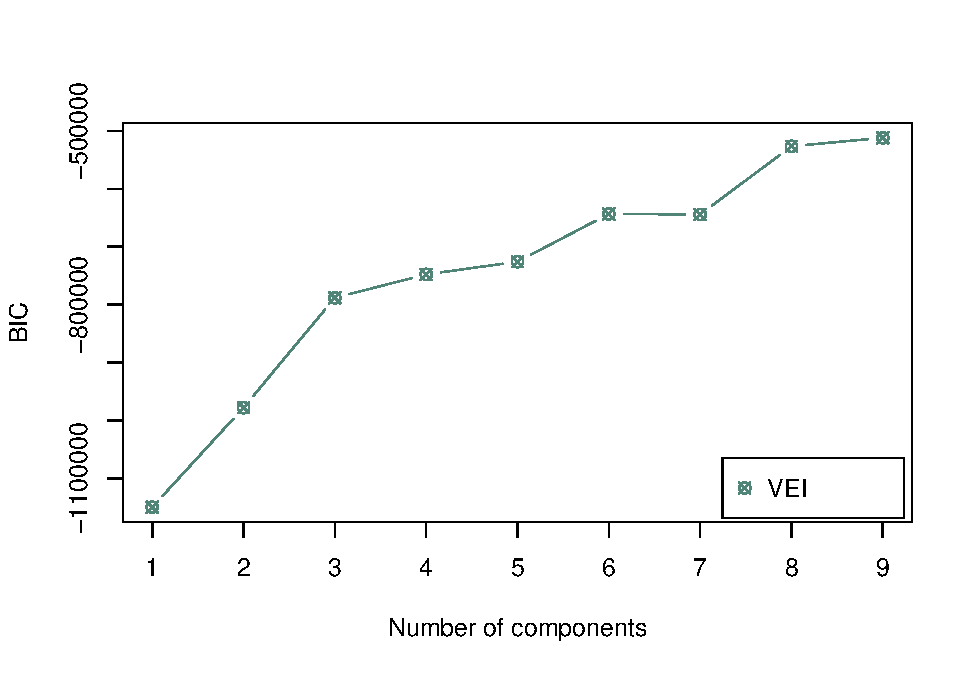
\includegraphics{customer_fitness_artigo_files/figure-latex/clusters-1.pdf}
\caption{\label{fig:clusters}Analysis number of clusters}
\end{figure}

\begin{figure}
\centering
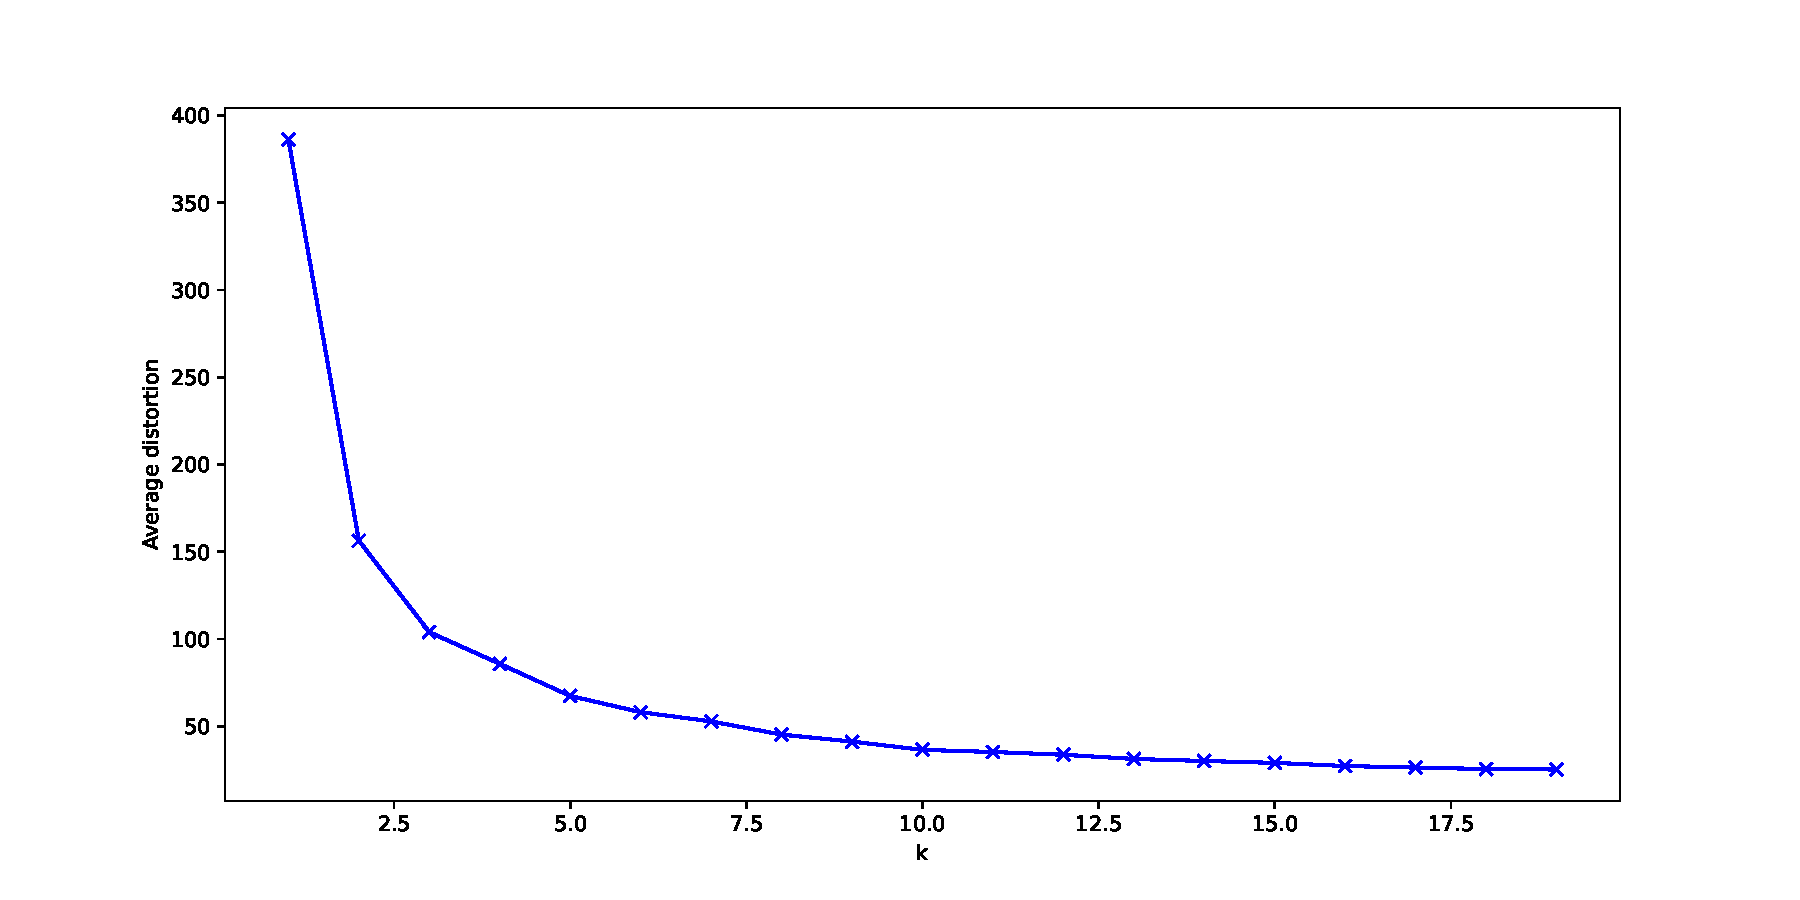
\includegraphics{customer_fitness_artigo_files/figure-latex/elbowCalculation-1.pdf}
\caption{\label{fig:elbowCalculation}Elbow analysis}
\end{figure}

The calculation of the clusters to each member in the dataset was developed considering,
7,6 and 4 clusters.
However after the executions KMeans only performed with 3 clusters.

\includegraphics{customer_fitness_artigo_files/figure-latex/kmeans PCA-3.pdf}

The model accuracy is very high in the first years. The prediction is very
similar to the actual value. The absolute error mean of
6 customers.

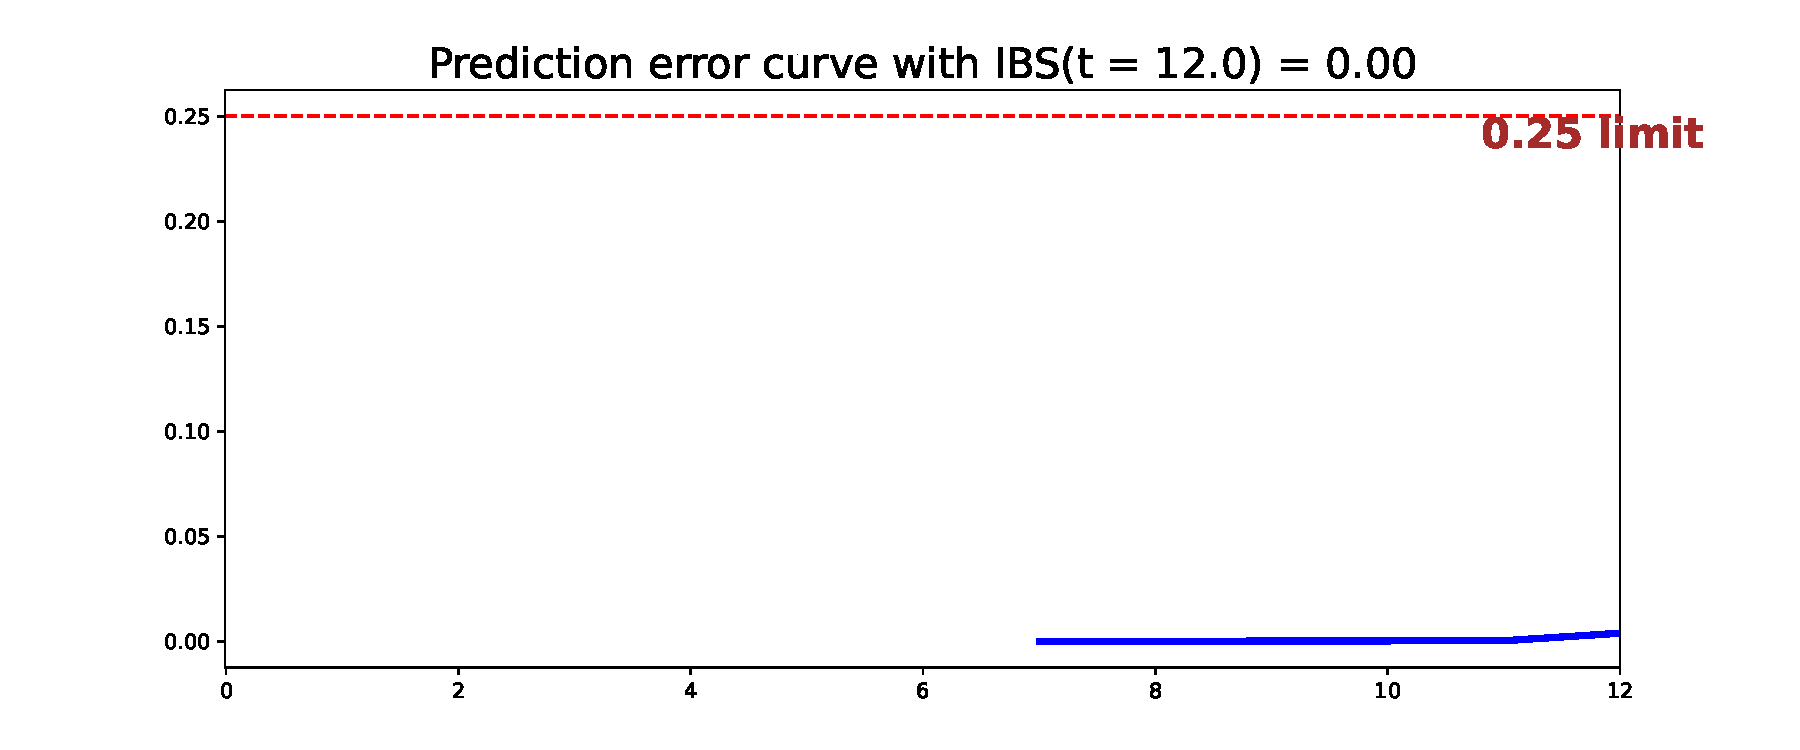
\includegraphics{customer_fitness_artigo_files/figure-latex/createModelClusters-5.pdf} 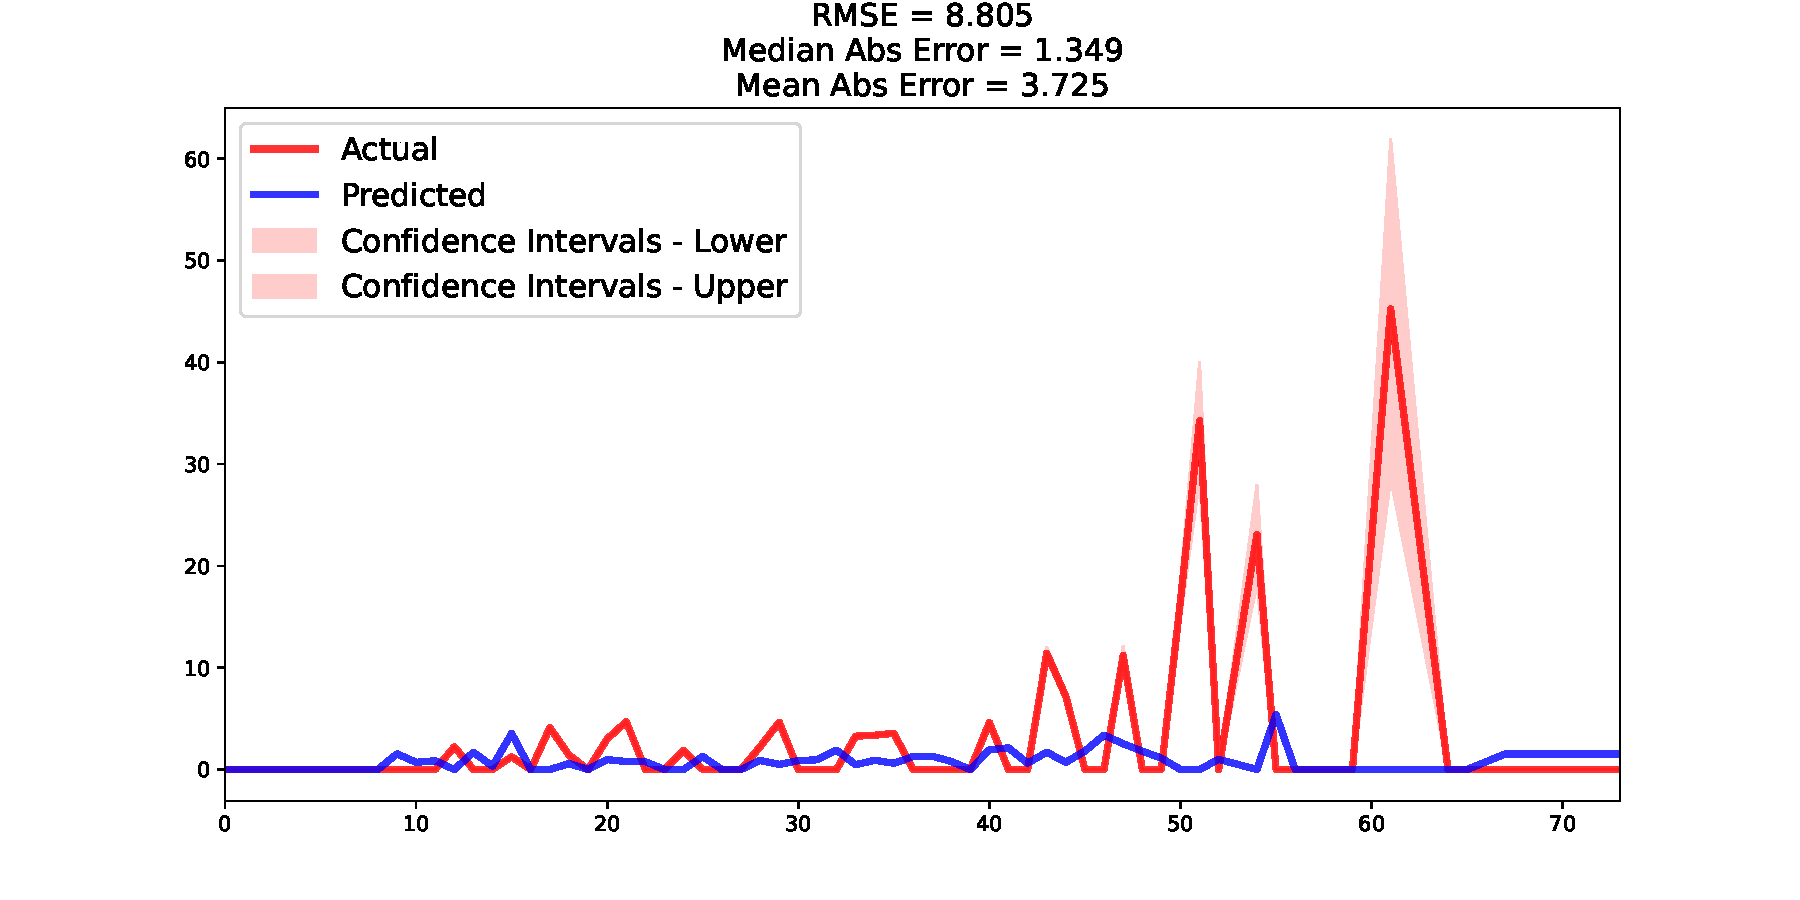
\includegraphics{customer_fitness_artigo_files/figure-latex/createModelClusters-6.pdf} 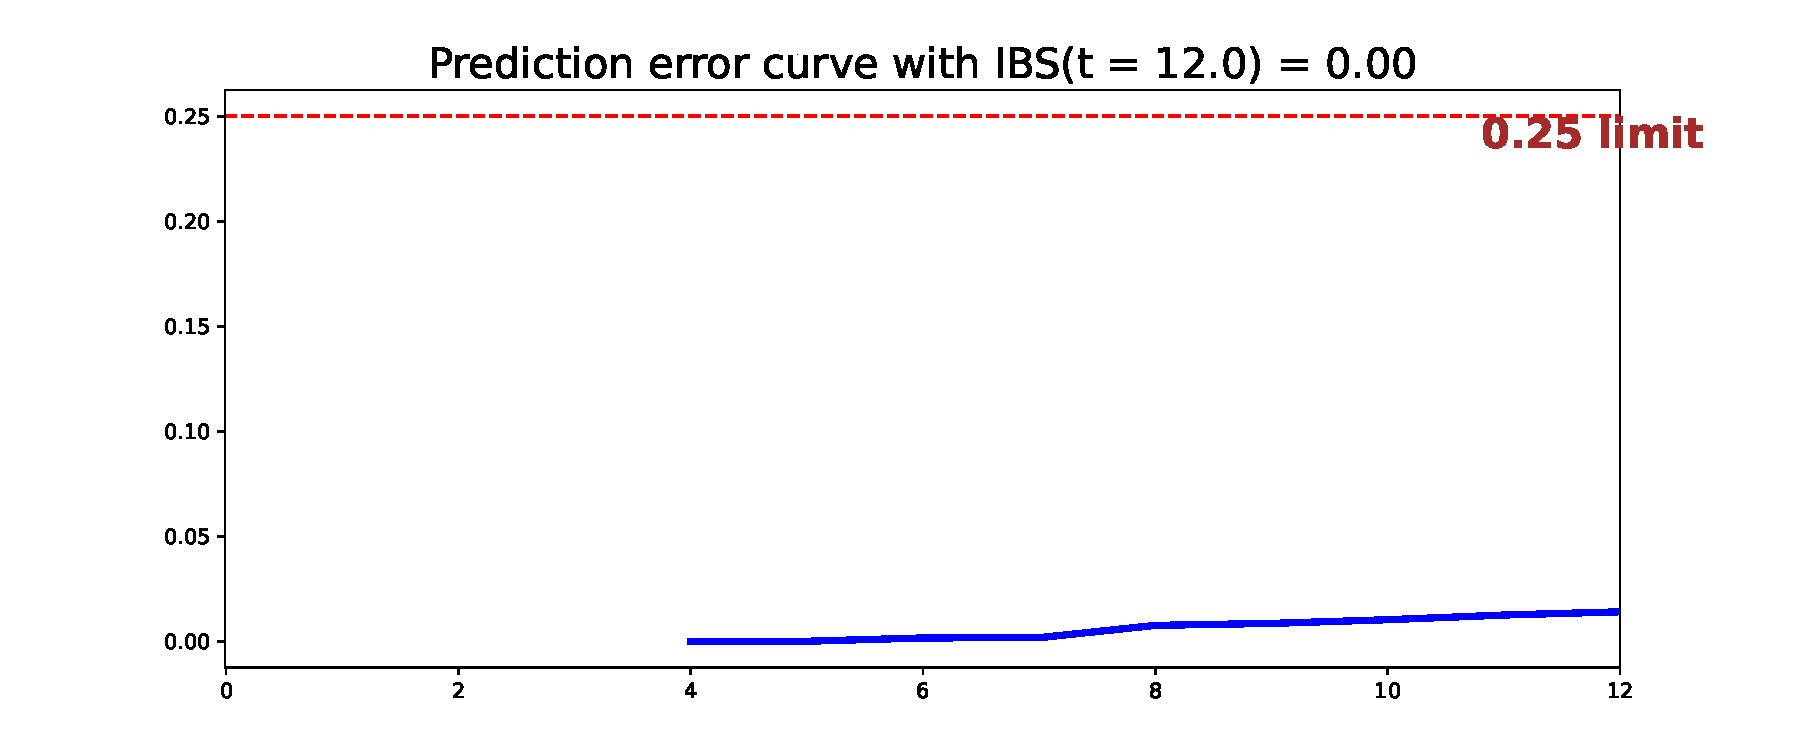
\includegraphics{customer_fitness_artigo_files/figure-latex/createModelClusters-7.pdf}

The performance of the cluster 1 the IBS presents an accuracy of 0.06
(figure \ref{fig:createModelCluster1IBS}) along all time.
The actual versus predicted model presents the actual and predicted customers which dropout during
the 40 months, which as an mean absolute error of 1.5 customers, the mean median absolute
error was 0.61 and the Root Mean Square Error of 2.8 (figure \ref{fig:createModelCluster1SF}).

The features importance in the survival model cluster 1 (table \ref{tab:summarytableCluster1})
identify the three most relevant features to predict survival \(maccess\),
\(tbilled\), and \(dayswfreq\). The features with lower relevance were \(freeuse\), \(sex\) and \(cfreq\).

\begin{figure}
\centering
\includegraphics{customer_fitness_artigo_files/figure-latex/createModelCluster1IBS-11.pdf}
\caption{\label{fig:createModelCluster1IBS}Model performance cluster 1}
\end{figure}

\begin{figure}
\centering
\includegraphics{customer_fitness_artigo_files/figure-latex/createModelCluster1SF-13.pdf}
\caption{\label{fig:createModelCluster1SF}Conditional survival forest cluster 1}
\end{figure}

\begin{table}

\caption{\label{tab:summarytableCluster1}Features importance in the survival model with cluster 1}
\centering
\begin{tabular}[t]{lrr}
\toprule
feature & importance & pct\_importance\\
\midrule
tbilled & 6.7827606 & 0.2644082\\
freeuse & 5.7521637 & 0.2242331\\
maccess & 4.4870321 & 0.1749152\\
dayswfreq & 3.9224018 & 0.1529046\\
nentries & 3.0360807 & 0.1183537\\
\addlinespace
cfreq & 0.8262370 & 0.0322087\\
age & 0.4607052 & 0.0179594\\
sex\_1 & 0.3852319 & 0.0150173\\
\bottomrule
\end{tabular}
\end{table}

The performance of the cluster 2 the IBS presents an accuracy along time 0.09
(figure \ref{fig:createModelCluster2IBS}) along all time.
The actual versus predicted model presents the actual and predicted customers which dropout during
the 40 months, which as an mean absolute error of 6.5 customers, the mean median absolute
error was 2.3 and the Root Mean Square Error of 11.79 (figure \ref{fig:createModelCluster2SF}).
The features importance in the survival model cluster 2 (table \ref{tab:summarytableCluster2})
identify the three most relevant features to predict survival \(dayswfreq\),
\(tbilled\), and \(freeuse\). The least relevant were \(nentries\), \(cfreq\), and \(age\).

\begin{figure}
\centering
\includegraphics{customer_fitness_artigo_files/figure-latex/createModelCluster2IBS-1.pdf}
\caption{\label{fig:createModelCluster2IBS}Model performance cluster 2}
\end{figure}

\begin{figure}
\centering
\includegraphics{customer_fitness_artigo_files/figure-latex/createModelCluster2SF-3.pdf}
\caption{\label{fig:createModelCluster2SF}Conditional survival forest cluster 2}
\end{figure}

The performance of the cluster 3 the IBS presents an accuracy along time 0.01
(figure \ref{fig:createModelCluster3IBS}) along all time.
The actual versus predicted model presents the actual and predicted customers which dropout during
the 40 months, which as an mean absolute error of 1.5 customers, the mean median absolute
error was 1.2 and the Root Mean Square Error of 2.08 (figure \ref{fig:createModelCluster3SF}).
The features importance in the survival model cluster 3 (table \ref{tab:summarytableCluster3})
identify the three most relevant features to predict survival \(tbilled\),
\(dayswfreq\), and \(nentries\).
The least relevant were \(sex\), \(age\), and \(cfreq\).

\begin{table}

\caption{\label{tab:summarytableCluster2}Features importance in the survival model with cluster 2}
\centering
\begin{tabular}[t]{lrr}
\toprule
feature & importance & pct\_importance\\
\midrule
tbilled & 6.6524419 & 0.2970936\\
maccess & 4.0288064 & 0.1799238\\
dayswfreq & 3.9304155 & 0.1755297\\
nentries & 2.7923452 & 0.1247043\\
freeuse & 2.4090838 & 0.1075881\\
\addlinespace
age & 1.4997470 & 0.0669777\\
sex\_1 & 1.0789000 & 0.0481829\\
cfreq & -0.6615769 & 0.0000000\\
\bottomrule
\end{tabular}
\end{table}

\begin{figure}
\centering
\includegraphics{customer_fitness_artigo_files/figure-latex/createModelCluster3IBS-1.pdf}
\caption{\label{fig:createModelCluster3IBS}Model performance cluster 3}
\end{figure}

\begin{figure}
\centering
\includegraphics{customer_fitness_artigo_files/figure-latex/createModelCluster3SF-3.pdf}
\caption{\label{fig:createModelCluster3SF}Conditional survival forest cluster 3}
\end{figure}

The features importance in the survival model (table \ref{tab:summarytableCluster3})
identify the three most relevant features to predict survival \(dayswfreq\),
\(tbilled\), and \(nentries\).

\begin{table}

\caption{\label{tab:summarytableCluster3}Features importance in the survival model with cluster 3}
\centering
\begin{tabular}[t]{lrr}
\toprule
feature & importance & pct\_importance\\
\midrule
tbilled & 3.7920500 & 0.3033014\\
nentries & 2.8590522 & 0.2286769\\
dayswfreq & 2.3304981 & 0.1864014\\
maccess & 1.8131070 & 0.1450186\\
age & 1.5533976 & 0.1242461\\
\addlinespace
sex\_1 & 0.1544767 & 0.0123556\\
freeuse & 0.0000000 & 0.0000000\\
cfreq & 0.0000000 & 0.0000000\\
\bottomrule
\end{tabular}
\end{table}

\hypertarget{model-comparison}{%
\subsubsection{Model Comparison}\label{model-comparison}}

Table \ref{tab:summarytable3} shows the performance of both approaches, with or without clusters.
The RMSE in the clusters 1, 2 and 3 is lower than not using clusters to predict dropout.
Overall the performance improved. The performance is also better using mean and median.

\begin{table}

\caption{\label{tab:summarytable3}Performance of prediction in each cluster}
\centering
\begin{tabular}[t]{llll}
\toprule
cluster & rmse & mean & median\\
\midrule
0 & 10.9534010098597 & 3.24949079763695 & 6.27043826620657\\
2 & 2.86277805553651 & 0.592331070836667 & 1.69865648584295\\
1 & 1.92696670365884 & 1.39451757989365 & 1.42197114146461\\
w/cluster & 13.8883596176347 & 3.75609199994054 & 7.22583527582812\\
\bottomrule
\end{tabular}
\end{table}

The model accuracy without clusters is very high with a root mean
square error of 13, the mean absolute error mean was 7.53 customers, and the median
absolute error was 4.04.
The model using clusters had an mean absolute error of 1.5 customers, the mean median absolute
error was 1.2 and the Root Mean Square Error of 2.08.
The performance using clusters improved significantly.

\hypertarget{conclusion}{%
\section{Conclusion}\label{conclusion}}

This paper investigated the customer dropout in a Health Club organization, using
a dynamic perspective that the dropout risk varies along the time.
Exploring two approaches, using a survival model based on random forests
with or without clusters.
The model using clusters allowed to combine the customers in different clusters,
an hybrid approach.
Based on this performance the proposed model using clusters allows to improve
the accuracy on the survival model allowing to target approaches considering
the timing when the dropout occurs, considering the clusters where the customer is.
Is very important for managers use this information to improve their retention
strategies.

\hypertarget{references}{%
\section*{References}\label{references}}
\addcontentsline{toc}{section}{References}

\hypertarget{refs}{}
\begin{CSLReferences}{1}{0}
\leavevmode\vadjust pre{\hypertarget{ref-akogul2016}{}}%
Akogul, Serkan and Murat Erisoglu. 2016. {``A Comparison of Information Criteria in Clustering Based on Mixture of Multivariate Normal Distributions.''} \emph{Mathematical and Computational Applications} 21(3):34.

\leavevmode\vadjust pre{\hypertarget{ref-Alboukaey_dynamic_2020}{}}%
Alboukaey, Nadia, Ammar Joukhadar, and Nada Ghneim. 2020b. {``Dynamic Behavior Based Churn Prediction in Mobile Telecom.''} \emph{Expert Systems with Applications} 162:113779.

\leavevmode\vadjust pre{\hypertarget{ref-alboukaey_dynamic_2020}{}}%
Alboukaey, Nadia, Ammar Joukhadar, and Nada Ghneim. 2020a. {``Dynamic Behavior Based Churn Prediction in Mobile Telecom.''} \emph{Expert Systems with Applications} 162:113779.

\leavevmode\vadjust pre{\hypertarget{ref-amin_customer_2017}{}}%
Amin, Adnan, Sajid Anwar, Awais Adnan, Muhammad Nawaz, Khalid Alawfi, Amir Hussain, and Kaizhu Huang. 2017. {``Customer Churn Prediction in the Telecommunication Sector Using a Rough Set Approach.''} \emph{Neurocomputing} 237:242--54.

\leavevmode\vadjust pre{\hypertarget{ref-ascarza_retention_2018}{}}%
Ascarza, Eva. 2018. {``Retention Futility: Targeting High-Risk Customers Might Be Ineffective.''} \emph{Journal of Marketing Research} 55(1):80--98.

\leavevmode\vadjust pre{\hypertarget{ref-Ascarza_Hardie_2013}{}}%
Ascarza, Eva and Bruce G. S. Hardie. 2013. {``A Joint Model of Usage and Churn in Contractual Settings.''} \emph{Marketing Science} 32(4):570--90.

\leavevmode\vadjust pre{\hypertarget{ref-Athanassopoulos_2000}{}}%
Athanassopoulos, Antreas D. 2000. {``Customer Satisfaction Cues to Support Market Segmentation and Explain Switching Behavior.''} \emph{Journal of Business Research} 47(3):191--207.

\leavevmode\vadjust pre{\hypertarget{ref-Bland_Altman_1998}{}}%
Bland, J. M. and D. G. Altman. 1998. {``Survival Probabilities (the Kaplan-Meier Method).''} \emph{BMJ (Clinical Research Ed.)} 317(7172):1572.

\leavevmode\vadjust pre{\hypertarget{ref-Breiman_2001}{}}%
Breiman, Leo. 2001. {``Random Forests.''} \emph{Machine Learning} 45(1):5--32.

\leavevmode\vadjust pre{\hypertarget{ref-burez_separating_2008}{}}%
Burez, J. and D. Vandenpoel. 2008. {``Separating Financial from Commercial Customer Churn: {A} Modeling Step Towards Resolving the Conflict Between the Sales and Credit Department.''} \emph{Expert Systems with Applications} 35(1-2):497--514.

\leavevmode\vadjust pre{\hypertarget{ref-Copeland_1923}{}}%
Copeland, Melvin T. 1923. {``Relation of Consumers' Buying Habits to Marketing Methods.''} \emph{Harvard Business Review} 1(3):282--89.

\leavevmode\vadjust pre{\hypertarget{ref-coussement_improving_2009}{}}%
Coussement, Kristof and Dirk Van den Poel. 2009. {``Improving Customer Attrition Prediction by Integrating Emotions from Client/Company Interaction Emails and Evaluating Multiple Classifiers.''} \emph{Expert Systems with Applications} 36(3, Part 2):6127--34.

\leavevmode\vadjust pre{\hypertarget{ref-Pilon_2021}{}}%
Davidson-Pilon, Cameron. 2021. \emph{CamDavidsonPilon/Lifelines}.

\leavevmode\vadjust pre{\hypertarget{ref-devriendt_why_2019}{}}%
Devriendt, Floris, Jeroen Berrevoets, and Wouter Verbeke. 2019. {``Why You Should Stop Predicting Customer Churn and Start Using Uplift Models.''} \emph{Information Sciences}.

\leavevmode\vadjust pre{\hypertarget{ref-Edward_Sahadev_2011}{}}%
Edward, Manoj and Sunil Sahadev. 2011. {``Role of Switching Costs in the Service Quality, Perceived Value, Customer Satisfaction and Customer Retention Linkage.''} \emph{Asia Pacific Journal of Marketing and Logistics} 23(3):327--45.

\leavevmode\vadjust pre{\hypertarget{ref-Ehrlinger_2016}{}}%
Ehrlinger, John. 2016. {``ggRandomForests: Exploring Random Forest Survival.''} \emph{arXiv:1612.08974 {[}Stat{]}}.

\leavevmode\vadjust pre{\hypertarget{ref-Fornell_Wernerfelt_1987}{}}%
Fornell, Claes and Birger Wernerfelt. 1987. {``Defensive Marketing Strategy by Customer Complaint Management: A Theoretical Analysis.''} \emph{Journal of Marketing Research} 24(4):337--46.

\leavevmode\vadjust pre{\hypertarget{ref-Fotso_others_2019}{}}%
Fotso, Stephane and others. 2019. \emph{PySurvival: Open Source Package for Survival Analysis Modeling}.

\leavevmode\vadjust pre{\hypertarget{ref-garcia_intelligent_2017}{}}%
García, David L., Angela Nebot, and Alfredo Vellido. 2017. {``Intelligent Data Analysis Approaches to Churn as a Business Problem: A Survey.''} \emph{Knowledge and Information Systems} 51(3):719--74.

\leavevmode\vadjust pre{\hypertarget{ref-gok_case_2015}{}}%
Gök, Mehmet, Tansel Özyer, and Jamal Jida. 2015. {``A {Case} {Study} for the {Churn} {Prediction} in {Turksat} {Internet} {Service} {Subscription}.''} Pp. 1220--24 in \emph{Proceedings of the 2015 {IEEE}/{ACM} {International} {Conference} on {Advances} in {Social} {Networks} {Analysis} and {Mining} 2015 - {ASONAM} '15}. Paris, France: ACM Press.

\leavevmode\vadjust pre{\hypertarget{ref-Gupta2006Modeling}{}}%
Gupta, Sunil, Dominique Hanssens, Bruce Hardie, Wiliam Kahn, V. Kumar, Nathaniel Lin, Nalini Ravishanker, and S. Sriram. 2006. {``Modeling Customer Lifetime Value.''} \emph{Journal of Service Research} 9(2):139--55.

\leavevmode\vadjust pre{\hypertarget{ref-hung_applying_2006}{}}%
Hung, Shin-Yuan, David C. Yen, and Hsiu-Yu Wang. 2006. {``Applying Data Mining to Telecom Churn Management.''} \emph{Expert Systems with Applications} 31(3):515--24.

\leavevmode\vadjust pre{\hypertarget{ref-Ishwaran_Kogalur_Blackstone_Lauer_2008}{}}%
Ishwaran, Hemant, Udaya B. Kogalur, Eugene H. Blackstone, and Michael S. Lauer. 2008. {``Random Survival Forests.''} \emph{The Annals of Applied Statistics} 2(3):841--60.

\leavevmode\vadjust pre{\hypertarget{ref-JafariMarandi_Denton_Idris_Smith_Keramati_2020}{}}%
Jafari-Marandi, Ruholla, Joshua Denton, Adnan Idris, Brian K. Smith, and Abbas Keramati. 2020. {``Optimum Profit-Driven Churn Decision Making: Innovative Artificial Neural Networks in Telecom Industry.''} \emph{Neural Computing and Applications} 32(18):14929--62.

\leavevmode\vadjust pre{\hypertarget{ref-Mellens_Dekimpe_Steenkamp_1996}{}}%
Mellens, Martin, Marnik Dekimpe, and JBEM Steenkamp. 1996. {``A Review of Brand-Loyalty Measures in Marketing.''} \emph{Review of Business and Economic Literature} 41(4):507--33.

\leavevmode\vadjust pre{\hypertarget{ref-perianez_churn_2016}{}}%
Perianez, Africa, Alain Saas, Anna Guitart, and Colin Magne. 2016. {``Churn {Prediction} in {Mobile} {Social} {Games}: {Towards} a {Complete} {Assessment} {Using} {Survival} {Ensembles}.''} Pp. 564--73 in \emph{2016 {IEEE} {International} {Conference} on {Data} {Science} and {Advanced} {Analytics} ({DSAA})}. Montreal, QC, Canada: IEEE.

\leavevmode\vadjust pre{\hypertarget{ref-Reichheld_1996}{}}%
Reichheld, Frederick F. 1996. {``Learning from Customer Defections.''} \emph{Harvard Business Review} 74(2):56--67.

\leavevmode\vadjust pre{\hypertarget{ref-risselada_staying_2010}{}}%
Risselada, Hans, Peter C. Verhoef, and Tammo H. A. Bijmolt. 2010. {``Staying {Power} of {Churn} {Prediction} {Models}.''} \emph{Journal of Interactive Marketing} 24(3):198--208.

\leavevmode\vadjust pre{\hypertarget{ref-routh_estimating_2020}{}}%
Routh, Pallav, Arkajyoti Roy, and Jeff Meyer. 2020. {``Estimating Customer Churn Under Competing Risks.''} \emph{Journal of the Operational Research Society} 1--18.

\leavevmode\vadjust pre{\hypertarget{ref-Saunders_1980}{}}%
Saunders, J. a. 1980. {``Cluster Analysis for Market Segmentation.''} \emph{European Journal of Marketing} 14(7):422--35.

\leavevmode\vadjust pre{\hypertarget{ref-Schober2018Survival}{}}%
Schober, Patrick and Thomas R. Vetter. 2018. {``Survival Analysis and Interpretation of Time-to-Event Data: The Tortoise and the Hare.''} \emph{Anesthesia and Analgesia} 127(3):792--98.

\leavevmode\vadjust pre{\hypertarget{ref-schwarz1978}{}}%
Schwarz, Gideon. 1978. {``Estimating the Dimension of a Model.''} \emph{The Annals of Statistics} 6(2):461--64.

\leavevmode\vadjust pre{\hypertarget{ref-scrucca2016}{}}%
Scrucca, Luca, Michael Fop, T. ,Brendan Murphy, and Adrian,E. Raftery. 2016. {``Mclust 5: Clustering, Classification and Density Estimation Using Gaussian Finite Mixture Models.''} \emph{The R Journal} 8(1):289.

\leavevmode\vadjust pre{\hypertarget{ref-Singer_Willett_1993}{}}%
Singer, Judith D. and John B. Willett. 1993. {``It's about Time: Using Discrete-Time Survival Analysis to Study Duration and the Timing of Events.''} \emph{Journal of Educational Statistics} 18(2):155--95.

\leavevmode\vadjust pre{\hypertarget{ref-Stensrud_Hernuxe1n_2020}{}}%
Stensrud, Mats J. and Miguel A. Hernán. 2020. {``Why Test for Proportional Hazards?''} \emph{JAMA} 323(14):1401--2.

\leavevmode\vadjust pre{\hypertarget{ref-vijaya_sivasankar_2019}{}}%
Vijaya, J. and E. Sivasankar. 2019. {``An Efficient System for Customer Churn Prediction Through Particle Swarm Optimization Based Feature Selection Model with Simulated Annealing.''} \emph{Cluster Computing} 22(S5):10757--68.

\leavevmode\vadjust pre{\hypertarget{ref-wangmachine2017}{}}%
Wang, Ping, Yan Li, and Chandan K. Reddy. 2017. {``Machine Learning for Survival Analysis: A Survey.''} \emph{arXiv:1708.04649 {[}Cs, Stat{]}}.

\end{CSLReferences}

\hypertarget{appendix-chunk-options}{%
\section*{Appendix: Chunk options}\label{appendix-chunk-options}}
\addcontentsline{toc}{section}{Appendix: Chunk options}

\hypertarget{software-versioning-r}{%
\subsection{Software versioning R}\label{software-versioning-r}}

\hypertarget{r}{%
\subsubsection{R}\label{r}}

\begin{Shaded}
\begin{Highlighting}[]
\FunctionTok{cat}\NormalTok{(}\FunctionTok{paste}\NormalTok{(}\StringTok{"\#"}\NormalTok{, }\FunctionTok{capture.output}\NormalTok{(}\FunctionTok{sessionInfo}\NormalTok{()), }\StringTok{"}\SpecialCharTok{\textbackslash{}n}\StringTok{"}\NormalTok{, }\AttributeTok{collapse  =} \StringTok{""}\NormalTok{))}
\end{Highlighting}
\end{Shaded}

\begin{verbatim}
## # R version 4.1.3 (2022-03-10) 
## # Platform: x86_64-w64-mingw32/x64 (64-bit) 
## # Running under: Windows 10 x64 (build 22622) 
## #  
## # Matrix products: default 
## #  
## # locale: 
## # [1] LC_COLLATE=Portuguese_Portugal.1252  LC_CTYPE=Portuguese_Portugal.1252    
## # [3] LC_MONETARY=Portuguese_Portugal.1252 LC_NUMERIC=C                         
## # [5] LC_TIME=Portuguese_Portugal.1252     
## #  
## # attached base packages: 
## # [1] stats     graphics  grDevices utils     datasets  methods   base      
## #  
## # other attached packages: 
## #  [1] mclust_5.4.10    labelled_2.9.1   kableExtra_1.3.4 gtsummary_1.6.0  
## #  [5] visdat_0.5.3     readxl_1.4.0     stargazer_5.2.3  reticulate_1.25  
## #  [9] ggplot2_3.3.6    dlookr_0.5.6     dplyr_1.0.9      
## #  
## # loaded via a namespace (and not attached): 
## #  [1] reactable_0.2.3     webshot_0.5.3       httr_1.4.3          
## #  [4] tools_4.1.3         utf8_1.2.2          R6_2.5.1            
## #  [7] rpart_4.1.16        colorspace_2.0-3    withr_2.5.0         
## # [10] tidyselect_1.1.2    gridExtra_2.3       curl_4.3.2          
## # [13] compiler_4.1.3      extrafontdb_1.0     cli_3.3.0           
## # [16] rvest_1.0.2         gt_0.6.0            xml2_1.3.3          
## # [19] labeling_0.4.2      bookdown_0.27       scales_1.2.0        
## # [22] mvtnorm_1.1-3       rappdirs_0.3.3      systemfonts_1.0.4   
## # [25] stringr_1.4.0       digest_0.6.29       rmarkdown_2.14      
## # [28] svglite_2.1.0       pkgconfig_2.0.3     htmltools_0.5.2     
## # [31] showtext_0.9-5      extrafont_0.18      fastmap_1.1.0       
## # [34] highr_0.9           htmlwidgets_1.5.4   rlang_1.0.2         
## # [37] rstudioapi_0.13     sysfonts_0.8.8      shiny_1.7.1         
## # [40] generics_0.1.2      farver_2.1.0        jsonlite_1.8.0      
## # [43] magrittr_2.0.3      Formula_1.2-4       Matrix_1.4-1        
## # [46] Rcpp_1.0.8.3        munsell_0.5.0       fansi_1.0.3         
## # [49] gdtools_0.2.4       partykit_1.2-15     lifecycle_1.0.1     
## # [52] stringi_1.7.6       yaml_2.3.5          inum_1.0-4          
## # [55] grid_4.1.3          hrbrthemes_0.8.0    promises_1.2.0.1    
## # [58] forcats_0.5.1       crayon_1.5.1        lattice_0.20-45     
## # [61] haven_2.5.0         splines_4.1.3       hms_1.1.1           
## # [64] knitr_1.39          pillar_1.7.0        glue_1.6.2          
## # [67] evaluate_0.15       pagedown_0.18       broom.helpers_1.7.0 
## # [70] vctrs_0.4.1         png_0.1-7           httpuv_1.6.5        
## # [73] Rttf2pt1_1.3.10     cellranger_1.1.0    gtable_0.3.0        
## # [76] purrr_0.3.4         tidyr_1.2.0         xfun_0.31           
## # [79] mime_0.12           libcoin_1.0-9       xtable_1.8-4        
## # [82] later_1.3.0         survival_3.3-1      viridisLite_0.4.0   
## # [85] tibble_3.1.7        showtextdb_3.0      ellipsis_0.3.2
\end{verbatim}

\begin{Shaded}
\begin{Highlighting}[]
  \CommentTok{\# or use message() instead of cat()}
\end{Highlighting}
\end{Shaded}


\end{document}
